% Chapter 06 - Postop CRP and complications

\chapter{An investigation into the relationship between postoperative systemic inflammation and complications after pancreaticoduodenectomy.}
\label{ch_survival}

\lhead{Chapter \ref{ch_survival}. \emph{Postoperative CRP and complications}} % This is for the header on each page - perhaps a shortened title

\clearpage
%----------------------------------------------------------------------------------------
\section{Introduction}
Pancreaticoduodenectomy is associated with significant morbidity in spite of advances in patient selection, perioperative care and surgical technique. Early identification of complications can help improve outcomes by better allocation of critical care resources as well as goal-directed therapy. Postoperative pancreatic fistula is one of the most dreaded complications after a pancreaticoduodenectomy and can lead to a cascade of other complications including delayed haemorrhage, infected intra-abdominal collections, delayed gastric emptying, prolonged hospitalisation and in some cases, death. The International Study Group for Pancreatic Fistula (ISGPF) have not only defined what constitutes a post-operative pancreatic fistula but have also graded the severity of this complication based on its impact on the management of the patient. However, these definitions are applied after the event and there is no clear way of predicting the severity of complications.

Postoperative CRP levels have been shown to predict infectious complications after colorectal surgery as well as oesophago-gastric surgery. It has been postulated that an unmitigated and exaggerated systemic inflammatory response in the early postoperative period is followed by a compensatory anti-inflammatory response that predisposes the patient to sepsis and impaired healing. The role of postoperative CRP in predicting the severity of complications after major pancreatic surgery has not been reported before. Stratifying patients based on the predicted severity of complications will allow identifying low risk patients who will be suitable to continue on enhanced recovery pathways and high risk patients who may require prolonged critical care, prolonged hospitalisation or further interventions.

The aim of this study was to investigate the association between postoperative systemic inflammation and severity of complications after pancreaticoduodenectomy.
 
 
\clearpage
\section{Methods}
\todo{Check dates for this study}
Patients who underwent pancreaticoduodenectomy between January 2008 and July 2012 were included in the study. Data were collected from a prospectively maintained database. All complications were discussed at a weekly meeting and prospectively recorded. Postoperative pancreatic fistula and post-pancreatectomy haemorrhage were graded according to the International Study Group classifications. All other complications were graded using the Clavien-Dindo system. Postoperative mortality was defined as death within 30-days of the operation or while still in hospital after the operation. Re-intervention in the form of radiological, endoscopic or surgical procedures was recorded prospectively. Preoperative blood results as well as postoperative blood results for the first 7 days after surgery were collected from the hospital laboratory databases. 

\subsection{Statistics}
SPSS version 22 was used for all analysis. ROC analysis was used to identify the optimum thresholds of CRP for predicting complications.
\todo{Complete this section - most of this can be modified from the stats sections in other chapters}



\clearpage
\section{Results}
One hundred and eighty patient (131 male) underwent pancreaticoduodenectomy during the study period. 

%CRP trends and pancreatic fistula
Postoperative CRP levels on days 2 through 7 were significantly higher in patients who developed a postoperative pancreatic fistula. However, CRP levels in the first postoperative week were not associated with the clinical severity of the pancreatic fistula. These results are presented in Table \ref{table:crp_comp_vs_POPF_ISGPS_p_values_only} and Fig. \ref{fig:crp_comp_crp_popf}. Fig. \ref{fig:crp_comp_crp_popf_isgps} shows that CRP levels were not significantly different between the different grades of pancreatic fistula while CRP levels in patients who did not develop a pancreatic fistula had significantly lower CRP levels.

%SPSS results and graphs are stored in crp_complications_graphs_etc.spv file

%==============================================================================
%CRP trends in a 2-panel figure and table showing p-values below it
\clearpage
\begin{figure}[htbp]
	\centering
	\begin{subfigure}{0.45\textwidth}
		\centering
		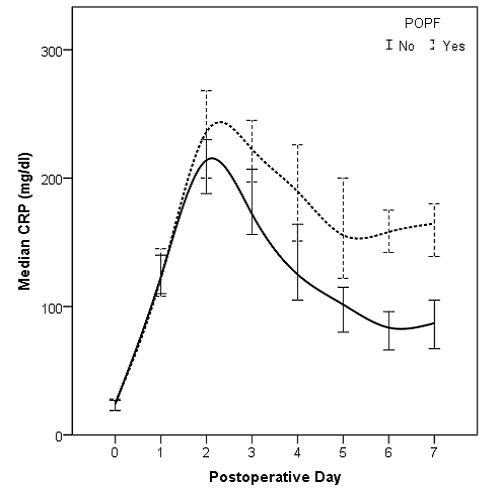
\includegraphics[width=\textwidth]{Figures/crp_comp_crp_popf_yes_no}
		\caption{POPF Absent vs. Any Grade}
		\label{fig:crp_comp_crp_popf_yes_no}
	\end{subfigure}
	\begin{subfigure}{0.45\textwidth}
		\centering
		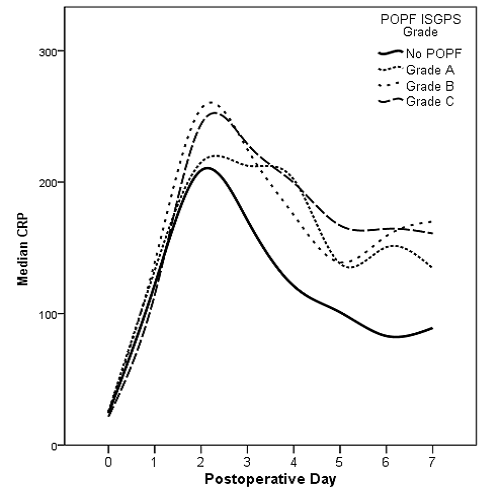
\includegraphics[width=\textwidth]{Figures/crp_comp_crp_popf_isgps}
		\caption{POPF ISGPS Grades}
		\label{fig:crp_comp_crp_popf_isgps}
	\end{subfigure}
	
	\caption{Serum CRP levels in the first week after pancreaticoduodenectomy in patients with postoperative pancreatic fistula (POPF).}
	\label{fig:crp_comp_crp_popf}
	
\end{figure}
%06/07/15 - Started this table
\begin{table}[h]
	\centering
	\caption{The relationship between CRP during the first postoperative week and post-operative pancreatic fistula (POPF) in patients undergoing pancreaticoduodenectomy.}
	\label{table:crp_comp_vs_POPF_ISGPS_p_values_only}
	\renewcommand{\arraystretch}{1.2} %Increases space between rows
	%\setlength{\tabcolsep}{9pt} %sets the space between columns
	\begin{tabular}{| c | c c c c |}
		\hline
		           &       \multicolumn{4}{c|}{POPF ISGPS Grades - \textit{p}}        \\
		Postop Day & No vs. Any Grade & No vs. A & A vs. B & B vs. C                 \\ \hline
		0          & 0.722            & 0.582    & 0.849   & 0.730                   \\
		1          & 0.242            & 0.331    & 0.740   & 0.295                   \\
		2          & 0.002            & 0.161    & 0.222   & 0.563                   \\
		3          & $<$0.001         & 0.022    & 0.602   & 0.530                   \\
		4          & $<$0.001         & 0.007    & 0.906   & 0.834                   \\
		5          & $<$0.001         & 0.035    & 0.611   & 0.959                   \\
		6          & $<$0.001         & 0.012    & 0.638   & 0.781                   \\
		7          & $<$0.001         & 0.006    & 0.235   & 0.356                   \\ \hline
		\multicolumn{5}{l}{\textit{p} - Mann-Whitney U test}                         \\
		\multicolumn{5}{l}{ISGPS - International Study Group for Pancreatic Surgery}	\\
				\multicolumn{5}{l}{POPF - Postoperative Pancreatic Fistula}
	\end{tabular}
	
	
\end{table}
%==============================================================================

%Ability of CRP to predict infectious complications in leak vs. no leak complications
%Rationale - POPF is diagnosed with a separate definition - ISGPS on Day 3. Therefore, there is no role for CRP in diagnosing POPF. Above results show that it does not discriminate between the grades either. Therefore, the following analysis is to find out if the first week CRP has any role in predicting other outcome measures.




%==============================================================================
%CRP trends in a 2-panel figure and table showing p-values below it
\clearpage
\begin{figure}[htbp]
	\centering
	\begin{subfigure}{0.45\textwidth}
		\centering
		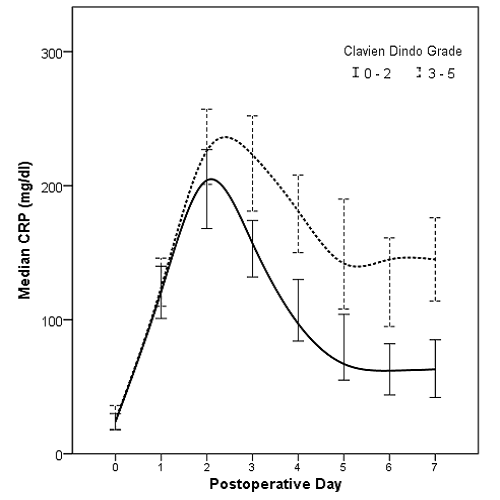
\includegraphics[width=\textwidth]{Figures/crp_comp_infectious_leak0}
		\caption{Patients with \textbf{\underline{no}} POPF}
		\label{fig:crp_comp_infectious_leak0}
	\end{subfigure}
	\begin{subfigure}{0.45\textwidth}
		\centering
		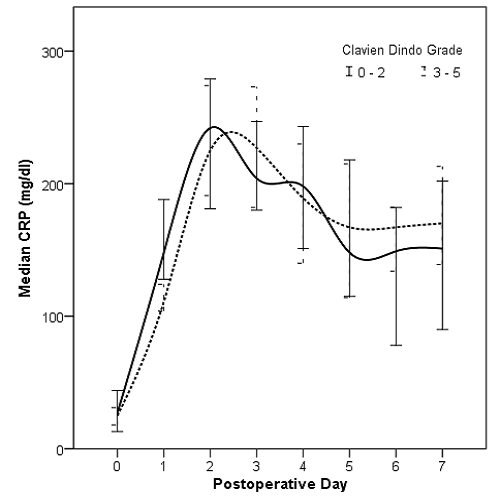
\includegraphics[width=\textwidth]{Figures/crp_comp_infectious_leak1}
		\caption{Patients with POPF}
		\label{fig:crp_comp_infectious_leak1}
	\end{subfigure}
	
	\caption{Relationship between postoperative CRP and clinically significant infectious complications in patients without (A) and with (B) POPF.}
	\label{fig:crp_comp_infectious_leak}
	
\end{figure}
%07/07/15 - Started this table
\begin{table}[h]
	\centering
	\caption{The relationship between postoperative CRP and infectious complications grouped by POPF. (Mann-Whitney U test)}
	\label{table:crp_comp_vs_infections_popf_y1n0}
	%\renewcommand{\arraystretch}{1.1} %Increases space between rows
	%\setlength{\tabcolsep}{9pt} %sets the space between columns
	\begin{tabular}{| c | c c c | c c c |}
		\hline
		           &       \multicolumn{3}{c}{POPF Absent}       &      \multicolumn{3}{c}{POPF Present}       \\
		           & \multicolumn{3}{c}{Infectious Complication} & \multicolumn{3}{c}{Infectious Complication} \\
		Postop Day & No          & Yes         & p               & No          & Yes         & p               \\
		           & (n=85)      & (n=41)      &                 & (n=19)      & (n=43)      &  \\ \hline
		0          & 24          & 25          & 0.379           & 27          & 25          & 0.629           \\
		           & (12 - 42)   & (14 - 41)   &                 & (13 - 44)   & (16 - 34)   &  \\
		1          & 122         & 123         & 0.667           & 148         & 116         & 0.038           \\
		           & (85 - 156)  & (87 - 148)  &                 & (114 - )    & (94 - 161)  &  \\
		2          & 204         & 218         & 0.203           & 242         & 228         & 0.919           \\
		           & (136 - 242) & (165 - 262) &                 & (181 - 279) & (186 - 296) &  \\
		3          & 157         & 213         & 0.011           & 206         & 226         & 0.846           \\
		           & (105 - 211) & (150 - 258) &                 & (180 - 297) & (175 - 281) &  \\
		4          & 97          & 173         & $<$0.001        & 214         & 190         & 0.559           \\
		           & (71 - 174)  & (118 - 216) &                 & (151 - 250) & (137 - 252) &  \\
		5          & 76          & 122         & $<$0.001        & 140         & 167         & 0.639           \\
		           & (40 - 129)  & (87 - 202)  &                 & (115 - 218) & (111 - 222) &  \\
		6          & 64          & 121         & $<$0.001        & 148         & 168         & 0.275           \\
		           & (31 - 133)  & (87 - 172)  &                 & (78 - 182)  & (109 - 224) &  \\
		7          & 62          & 141         & $<$0.001        & 158         & 167         & 0.644           \\
		           & (25 - 106)  & (90 - 190)  &                 & (90 - 231)  & (101 - 226) &  \\ \hline
		\multicolumn{7}{l}{Values are median (inter-quartile range.)}                                          \\
		\multicolumn{7}{l}{p - Mann-Whitney U test)}
	\end{tabular}
\end{table}
%==============================================================================



\clearpage
\section{Discussion}